\documentclass[ignorenonframetext,]{beamer}
\usetheme{AnnArbor}
\usecolortheme{dolphin}
\usefonttheme{structurebold}
\usepackage{amssymb,amsmath}
\usepackage{ifxetex,ifluatex}
\usepackage{fixltx2e} % provides \textsubscript
\usepackage{lmodern}
\ifxetex
  \usepackage{fontspec,xltxtra,xunicode}
  \defaultfontfeatures{Mapping=tex-text,Scale=MatchLowercase}
  \newcommand{\euro}{€}
\else
  \ifluatex
    \usepackage{fontspec}
    \defaultfontfeatures{Mapping=tex-text,Scale=MatchLowercase}
    \newcommand{\euro}{€}
  \else
    \usepackage[T1]{fontenc}
    \usepackage[utf8]{inputenc}
      \fi
\fi
\IfFileExists{upquote.sty}{\usepackage{upquote}}{}
% use microtype if available
\IfFileExists{microtype.sty}{\usepackage{microtype}}{}
\usepackage{url}
\usepackage{letltxmacro}
\makeatletter
\def\maxwidth{\ifdim\Gin@nat@width>\linewidth\linewidth\else\Gin@nat@width\fi}
\def\maxheight{\ifdim\Gin@nat@height>\textheight0.8\textheight\else\Gin@nat@height\fi}
\makeatother
\AtBeginDocument{
  \LetLtxMacro\Oldincludegraphics\includegraphics
  \renewcommand{\includegraphics}[2][]{%
    \Oldincludegraphics[#1,width=\maxwidth,height=\maxheight,keepaspectratio]{#2}}
}

% Comment these out if you don't want a slide with just the
% part/section/subsection/subsubsection title:
\AtBeginPart{
  \let\insertpartnumber\relax
  \let\partname\relax
  \frame{\partpage}
}
\AtBeginSection{
  \let\insertsectionnumber\relax
  \let\sectionname\relax
  \frame{\sectionpage}
}
\AtBeginSubsection{
  \let\insertsubsectionnumber\relax
  \let\subsectionname\relax
  \frame{\subsectionpage}
}

\setlength{\parindent}{0pt}
\setlength{\parskip}{6pt plus 2pt minus 1pt}
\setlength{\emergencystretch}{3em}  % prevent overfull lines
\setcounter{secnumdepth}{0}

\title{Reproducible Research}
\author{Andrew Caines \textbar{} ALTA-DTAL \textbar{} apc38}
\date{23 February 2015}

\begin{document}
\frame{\titlepage}

\begin{frame}{Overview}

\begin{itemize}[<+->]
\itemsep1pt\parskip0pt\parsep0pt
\item
  reproducible research
\item
  case studies
\item
  R Markdown
\end{itemize}

\end{frame}

\begin{frame}{Reproducible research}

\begin{itemize}[<+->]
\itemsep1pt\parskip0pt\parsep0pt
\item
  available data
\item
  available, functioning code
\item
  Reproducibility movement
\end{itemize}

\end{frame}

\begin{frame}{Why reproducible research?}

\begin{itemize}[<+->]
\itemsep1pt\parskip0pt\parsep0pt
\item
  incremental Science
\item
  collaborate with anyone anywhere
\item
  avoid scandals: don't end up in
  \href{http://retractionwatch.com/}{Retraction Watch}
\item
  be good and keep up / go with the flow: e.g.
  \href{http://www.theguardian.com/science/head-quarters/2014/jan/24/the-changing-face-of-psychology}{Psychology},
  \href{http://journals.cambridge.org/action/displayIssue?jid=PSC\&volumeId=47\&seriesId=0\&issueId=01}{PolSci},
  \href{http://www.siam.org/news/news.php?id=2078}{CompSci}
\end{itemize}

\end{frame}

\begin{frame}{What is reproducibility?}

\begin{itemize}[<+->]
\itemsep1pt\parskip0pt\parsep0pt
\item
  paper + supplementary information / external website
\item
  e.g.1:
  \href{http://opendata.uit.no/dvn/faces/study/StudyPage.xhtml?studyId=19}{UiT
  Dataverse}
\item
  e.g.2:
  \href{http://www.pnas.org/content/early/2015/02/04/1411678112}{Dodds
  et al}
\item
  e.g.3: \href{http://www.martijnwieling.nl/publications}{Wieling}
\end{itemize}

\end{frame}

\begin{frame}{Break}

\begin{itemize}[<+->]
\itemsep1pt\parskip0pt\parsep0pt
\item
  questions?
\item
  next: R Markdown
\end{itemize}

\end{frame}

\begin{frame}{What is R Markdown?}

\begin{itemize}[<+->]
\itemsep1pt\parskip0pt\parsep0pt
\item
  source file / output file paradigm (cp LaTeX, HTML, markdown)
\item
  plain text file (.Rmd), rendered by R
\item
  markdown = plain-text authoring syntax, increasingly popular
  (e.g.~GitHub)
\item
  R Markdown = implementation of markdown, can process output from R
\item
  uses \texttt{knitr} package (successor to \texttt{Sweave}) and
  `Pandoc' text file conversion program
\item
  can produce HTML, PDF and Word documents
\end{itemize}

\end{frame}

\begin{frame}{What is R Markdown?}

\begin{itemize}[<+->]
\itemsep1pt\parskip0pt\parsep0pt
\item
  \textbf{simple syntax}: shallow learning curve
\item
  \textbf{human-readable}: emphasis on communication and clarity, rather
  than technique and complexity
\item
  \textbf{transparent formatting}: wysiwyg
\item
  \textbf{embedded computation}: share with collaborators, reviewers,
  colleagues, students, critics
\end{itemize}

\end{frame}

\begin{frame}{What is R Markdown?}

\begin{quote}
\ldots{} integrating source code, statistical output, and text in R
Markdown is \textbf{a model of reproducibility}.
\end{quote}

\begin{quote}
Such transparency facilitates comprehension, defensibility, and further
research or testing.
\end{quote}

\begin{quote}
R Markdown helps to bring the vision for reproducibility in statistical
analysis articulated by Gentleman \& Temple Lang {[}2004{]} to reality.
\end{quote}

\begin{itemize}[<+->]
\itemsep1pt\parskip0pt\parsep0pt
\item
  \href{http://arxiv.org/abs/1501.01613}{Udwin \& Baumer 2015, `R
  Markdown', arXiv.org}
\end{itemize}

\end{frame}

\begin{frame}{What is R Markdown?}

\begin{quote}
This vision --- in which the barriers to verify another's statistical
computations from start to finish are low --- is the intellectual
descendant of Claerbout {[}1994{]}, Buckheit \& Donoho {[}1995{]}, and
began with Knuth {[}1984{]}, the creator of TEX.
\end{quote}

\begin{quote}
Moreover, R Markdown is dynamic: each time the document is rendered, the
commands therein are run anew. If data are altered or different data are
called in advance of rendering, then the output is dependent and
calculated accordingly.
\end{quote}

\begin{itemize}[<+->]
\itemsep1pt\parskip0pt\parsep0pt
\item
  \href{http://arxiv.org/abs/1501.01613}{Udwin \& Baumer 2015, `R
  Markdown', arXiv.org}
\end{itemize}

\end{frame}

\begin{frame}{How to use R Markdown}

\begin{block}{installation}

\begin{itemize}[<+->]
\itemsep1pt\parskip0pt\parsep0pt
\item
  \texttt{install.packages(\textquotesingle{}rmarkdown\textquotesingle{})}
\item
  \texttt{library(rmarkdown)}
\end{itemize}

\end{block}

\end{frame}

\begin{frame}{How to use R Markdown}

\begin{block}{simple syntax, human-readable, transparent formatting}

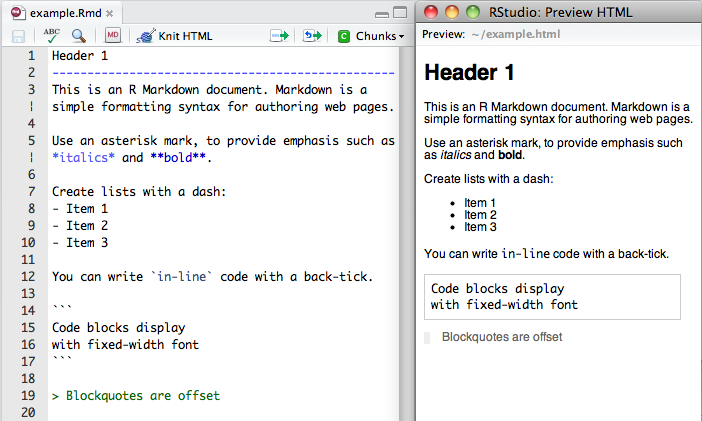
\includegraphics{images/markdownOverview.png}

\end{block}

\end{frame}

\begin{frame}{How to use R Markdown}

\begin{block}{embedded computation}

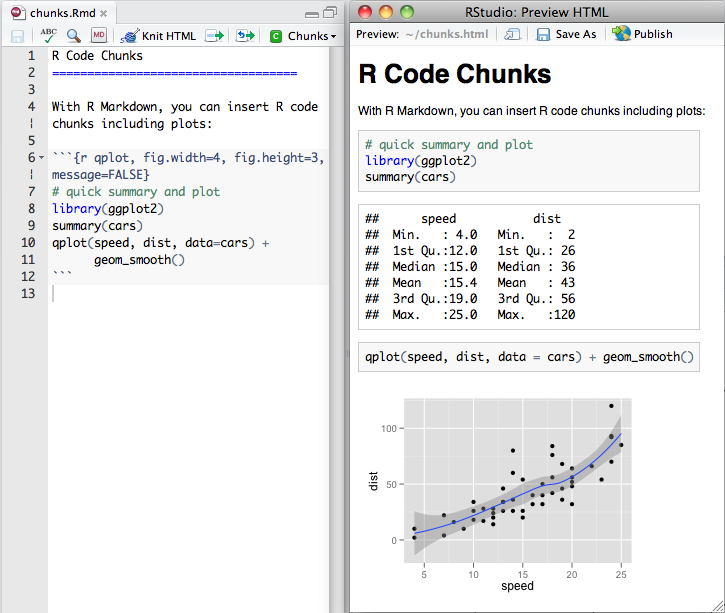
\includegraphics{images/markdownChunk.png}

\end{block}

\end{frame}

\begin{frame}{R Markdown and Reproducibility}

\begin{itemize}[<+->]
\itemsep1pt\parskip0pt\parsep0pt
\item
  example 1:
  \href{https://github.com/cainesap/replication/blob/master/slides.Rmd}{Beamer
  presentation}
\item
  example 2:
  \href{https://raw.githubusercontent.com/cainesap/replication/master/html_doc.Rmd}{HTML
  output demo}
\item
  example 3:
  \href{https://raw.githubusercontent.com/cainesap/replication/master/shiny_doc.Rmd}{interactive
  documents with Shiny}
\item
  example 4:
  \href{http://openscience.uni-leipzig.de/index.php/mr2/article/view/41}{paper
  packages}
\end{itemize}

\end{frame}

\begin{frame}{End}

\begin{block}{useful links}

\begin{quote}
\href{http://rmarkdown.rstudio.com/}{RStudio: R Markdown}
\href{http://arxiv.org/abs/1501.01613}{Udwin \& Baumer arXiv.org paper}
\href{http://shiny.rstudio.com/articles/interactive-docs.html}{Shiny \&
R Markdown} \href{https://github.com/cainesap/replication}{my GitHub
`replication' repo}
\end{quote}

\end{block}

\begin{block}{contact me}

\begin{itemize}
\itemsep1pt\parskip0pt\parsep0pt
\item
  apc38
\item
  \href{http://apc38.user.srcf.net/}{my website}
\item
  {[}@cainesap{]}(\url{https://twitter.com/cainesap})
\end{itemize}

\end{block}

\end{frame}

\end{document}
